\section{Methods} \label{sec:methods}

TODO
introduce two high-level methods for learning evolvable genotype-phenotype mappings
discuss two problem domains used to demonstrate these methods and the specific implementation of the methods in each of those domains
overview evolvability signature for the unfamiliar

\subsection{Learning an Evolvable Genotype-Phenotype Mapping}

The pair of proposed techniques to automatically learn evolvable genotype-phenotype mappings are based on autoencoders trained to encode phenotypes taken from local fitness peaks spread throughout an evolutionary search space.
(These phenotypes are gathered by evolving a large number of replicate direct-encoded populations and retaining champion individuals from each population).

\begin{figure}
  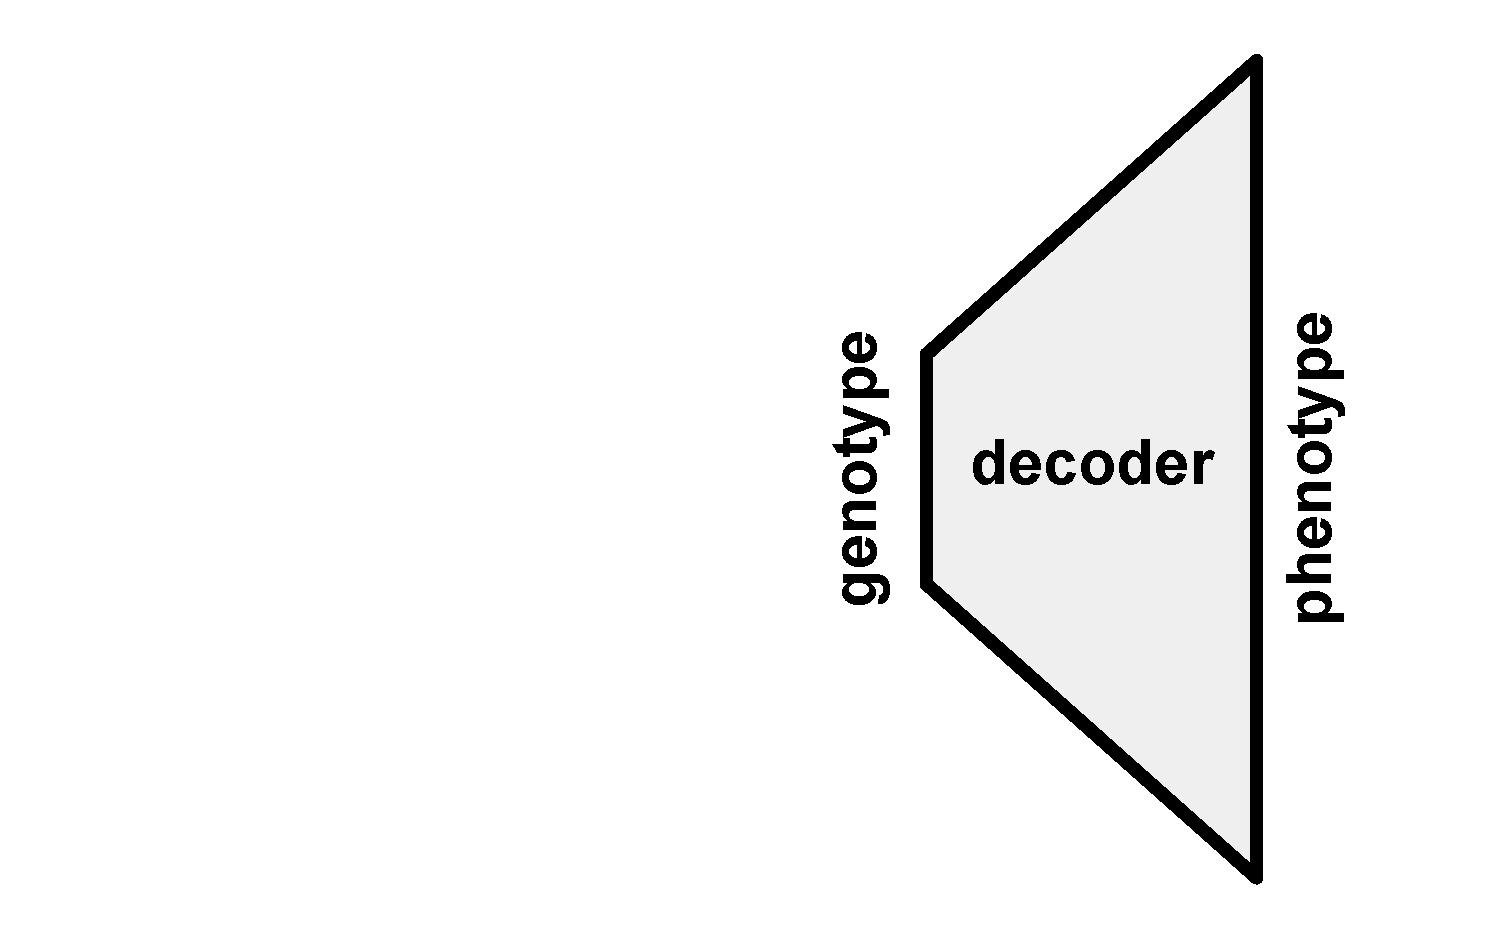
\includegraphics[width=\linewidth]{img/bottleneck_map}
  \caption{Schematic of a genotype-phenotype map constructed with a bottlenecked autoencoder.}
  \label{fig:bottleneck_map}
\end{figure}


The first approach, the bottleneck map, exploits just the decoder portion of the bottleneck autoencoder.
The decoder serves as the genotype-phenotype map so the genotype is now in the bottleneck vector space while the phenotype remains in the same vector space as before.
The idea of this approach is that, because the bottleneck provides a compact representation of those high-fitness phenotypes, using the decoder as a genotype-phenotype mapping will readily allow mutation to move the phenotype between otherwise distant fitness peaks.
This approach is illustrated in Figure \ref{fig:bottleneck_map}.

\begin{figure}
  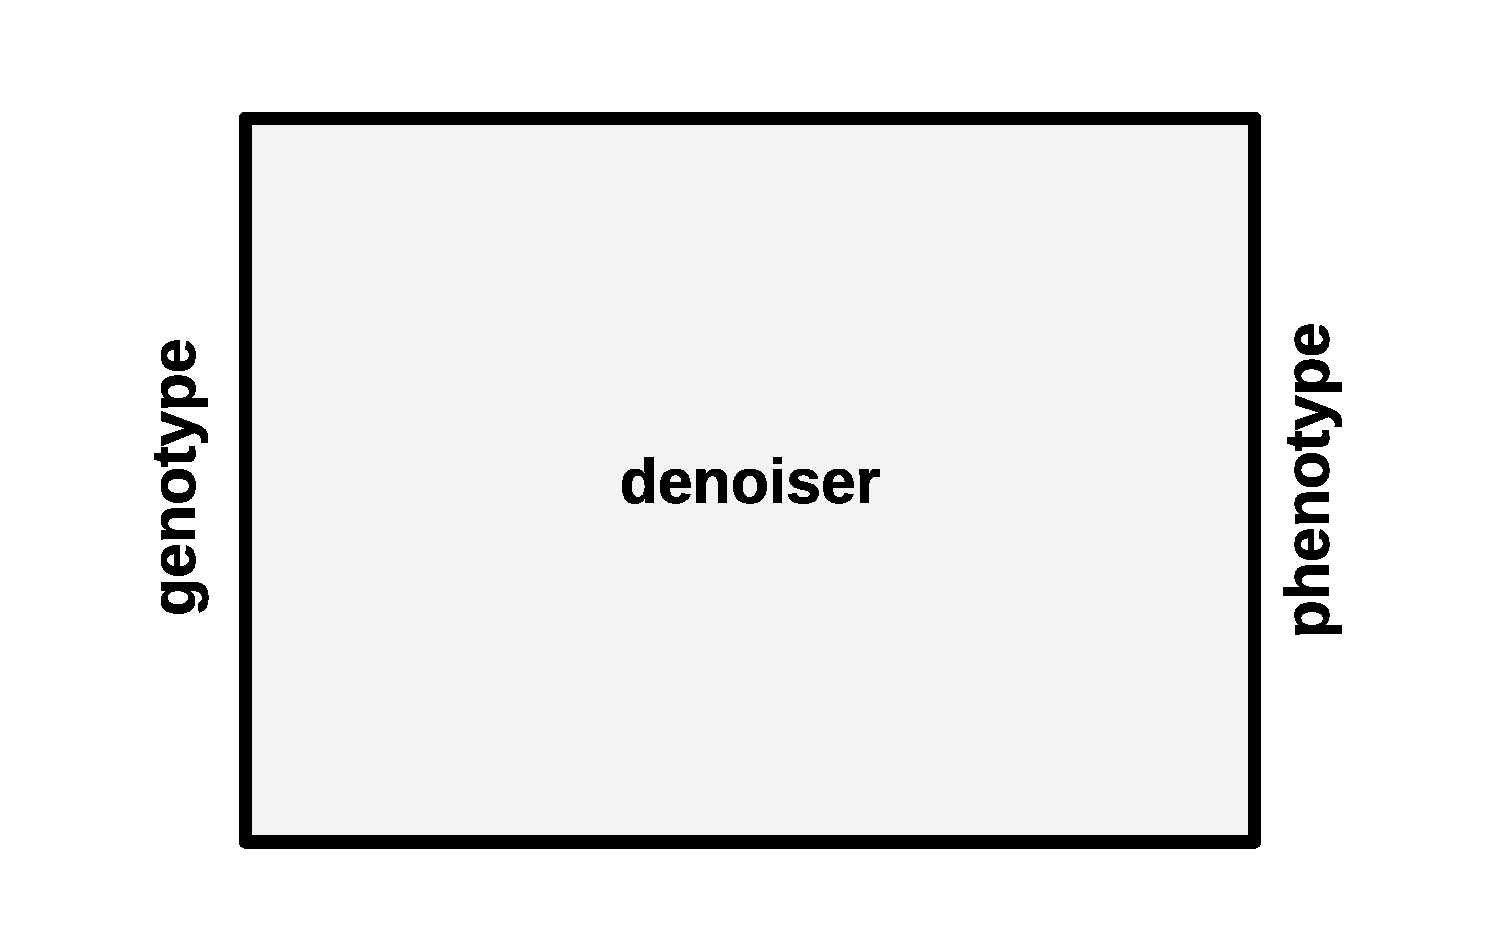
\includegraphics[width=\linewidth]{img/denoiser_map}
  \caption{
    Schematic of a genotype-phenotype map constructed with a denoising autoencoder.
  }\label{fig:denoiser_map}
\end{figure}


The second approach, the denoiser map, employs the entire denoising autoencoder would be used as the genotype-phenotype mapping.
Note that the genotype and phenotype remain in the same, equivalent vector spaces.
The idea of this design is that mutations that would otherwise be deleterious will be interpreted as noise and prevented from being expressed by the genotype-phenotype mapping.
Effectively, this mapping should flatten out the valleys between local fitness peaks to allow evolution to more readily drift between those local fitness peaks.
This approach is illustrated in Figure \ref{fig:denoiser_map}.


A pair of experiments was performed to assess the evolvability of the denoising autoencoder and the bottleneck decoder genotype-phenotype maps in relation to the direct genotype-phenotype map.
A high-level overview of these experiments is provide immediately below.
Methodological details can be found in the subsequent subsections.

First, in evolvability signature experiments the novelty and deleteriousness of mutation was assessed under these three genotype-phenotype maps.
Populations of 300 individuals were evolved using a particular map for 50 generations.
Then, the individual with the best fitness score over those 50 generations was isolated.
Mutant offspring of that individual were assessed for phenotypic novelty in relation to their parent and fitness score.
Phenotypic novelty was assessed as the euclidean distance between a parent phenotype $\vec{p}$ and a child phenotype $\vec{x}$.
Fitness was calculated according to the same criteria used during the 50 generations of evolution (described below).
Forty replicate evolutionary runs were performed for each genotype-phenotype map.
For each replicate run, 10,000 mutant offspring of the sampled champion were assessed.
The novelty and fitness scores of these mutant offspring (pooled over all 40 replicate runs) was used to generate the evolvability signatures presented in Section \ref{sec:results} \cite{tarapore2015evolvability}.

Second, experiments were performed to assess the ability of the three genotype-phenotype maps to facilitate traversal of the evolutionary search space in response to a selective pressure.
Specifically, a selective pressure for short (i.e. zero) table height was added.
Table height is calculated as the mean leg length of a table.
For each map, three replicate populations of 300 individuals were evolved for 5,000 generations.
These populations were initialized to have table height of approximately 1,000.
Response to selective pressure for short table height was assessed by tracking mean table height of the populations generation-by-generation.

\subsection{Bottleneck Autoencoder ANN Architecture and Training}

The bottleneck autoencoder was composed of two architectural components: an encoder and a decoder.
The encoder consisted of a 100-to-1 fully-connected linear layer with bias.
The decoder consisted of a 1-to-100 fully-connected linear layer with bias.
Thus, the bottleneck consisted of 1 float value.

The was network was trained for 200 epochs by stochastic gradient descent with parameter settings:
\begin{itemize}
  \item learning rate: $1^{-3}$
  \item momentum: $0.7$
  \item batch size: $16$
\end{itemize}
Loss was defined as mean square error of the difference between the presented phenotype and output (the reconstructed phenotype).

Training data for the bottleneck encoder was generated from 250 populations of 300 individuals evolved with direct genotype-phenotype map.
Initial leg lengths of each separate population were taken from a Gaussian random walk seeded uniformly between $0$ and $1000$ with $\mu = 0, \sigma = 1.0$ where each 100 consecutive values was taken as the initial leg lengths of a particular individual.
This step was performed to ensure that the 250 populations were well-spread throughout the phenotype space.
The 250 populations were evolved separately for 50 generations using the operators and settings described for the direct encoding for the evolvability signature experiments.
The 7500 phenotypes --- vectors of 100 float values --- present in the populations after 50 generations of evolution were taken as training data.
Leg lengths in the phenotypes were normalized to the range $(0,1)$ for the training process.

\subsection{Denoising Autoencoder ANN Architecture and Training}

The denoising autoencoder consisted of a 100-to-100 fully-connected linear layer without bias.

The was network was trained for 2500 epochs by stochastic gradient descent with parameter settings:
\begin{itemize}
  \item learning rate: $1^{-4}$
  \item momentum: $0.9$
  \item batch size: $2048$
\end{itemize}
Model parameters were initialized uniformly between $0.005$ and $0.015$.
During training, parameters were clamped in the range $(0,1)$.
During the training process, Gaussian noise with $\mu = 0, \sigma = 0.025$ was introduced to the input presented to the autoencoder.
Loss was defined as mean square error of the difference between the original phenotype without Gaussian noise and output (the reconstructed phenotype).

The same training data generated for the bottleneck autoencoder was used to train the denoising encoder.

\subsection{Genotype-Phenotype Maps}

Three genotype-phenotype maps were used: the direct genotype-phenotype map, the bottleneck decoder encoding, and the denoising encoding.
In these experiments, the phenotype is 100 floats (representing 100 individual leg lengths).
Thus, for all three maps, the phenotype space is $\mathcal{R}^{100}$.

The direct genotype-phenotype map is the identity function so under the direct map, the genotype space is $\mathcal{R}^{100}$.

Under the bottleneck map, just the decoder component of the full bottleneck autoencoder is used as the genotype-phenotype map.
The bottleneck autoencoder used in these experiments narrows down to a single node layer, so under this map the genotype space is $\mathcal{R}$.

Under the denoising encoding, the full denoising autoencoder is used.
The shape of input to the denoising autoencoder is identical to the shape of the phenotype (a hundred-float vector), so under this map the genotype space is $\mathcal{R}^{100}$.

\subsection{Operators}

For all experiments, tournament selection with $k = 5$ was used.
Two-point crossover was also used in all experiments.
(Note, though, that when the bottleneck genotype-phenotype is was employed the genotype is a member of $\mathcal{R}$ so crossover has no effect.)
All offspring engaged in crossover with one other individual with a probability $0.5$.
Mutation was performed by site-wise Gaussian perturbation of the genome.
For evolvability signature experiments, mutation of genome elements was $\mu=0, \sigma=0.1$ with a per-individual probability of $0.2$ and a subsequent per-site probability of $0.01$.
For response to selection experiments, mutation of genome elements was $\mu=0, \sigma=0.1$ with a per-individual probability of $0.2$ and a per-site probability of $0.2$.
(For all experiments with the bottleneck map, a per-site probability of $1$ $\sigma=0.1$ was employed.)

These particular operators were used due to their easy accessibility in DEAP.
As these experiments were demonstrative instead of applied, the primary criteria
for operators and parameters needed to meet was simply not being obscure enough to distract from the new genotype-phenotype mapping techniques being demonstrated.
It would be beneficial to repeat these experiments with other operator and parameter choices popular in the literature and in applied use to investigate the generalizability of those new techniques.


\subsection{Evaluation Functions}

For evolvability signature experiments, ``level-ness'' was the sole criterion determining fitness score.
For a phenotype $\vec{x}$, the fitness score was computed as
\begin{align*}
-\sigma(\vec{x})
\end{align*}
where $\sigma$ represents calculation of standard deviation.
Note that in all experiments performed, selection was performed to maximize (not minimize) fitness score.
Under this criterion, each level table of a particular height is a local fitness peak because any single-site mutation increases the leg height variance.
This fitness criteria was chosen for evolvability signature experiments because of its ruggedness.

For response to selection experiments, the ``level-ness'' and absolute height of a table were both factored into the fitness score.
For a phenotype $\vec{x}$, the fitness score was computed as
\begin{align*}
-\sigma(\vec{x}) - |\mu(\vec{x})/10|
\end{align*}
where $\sigma$ represents calculation of standard deviation and $\mu$ represents calculation of mean.
Under this criterion, a selection pressure for short tables is applied.
The global fitness score peak is the table with all legs length 0.
However, the phenotypic fitness landscape remains rugged with local peaks occurring as before at level tables.
Thus, the ability of genotype-phenotype map to facilitate evolution will be reflected by the ability of a population to escape local fitness peaks and progress towards the global fitness peak.

\subsection{Implementation}

The evolutionary computing components of this project were implemented using the Distributed Evolutionary Algorithms for Python package, which allows for rapid prototyping and extreme flexibility \cite{fortin2012deap}.
The artificial neural network autoencoder components of this project were implemented using PyTorch, a Python-based deep learning framework \cite{paszke2017pytorch}.

Experiments were run on a PC (no GPU).
In total, the experiments reported used approximately 12 hours of compute time.

\subsection{$n$-legged Table Problem}
TODO

\subsection{Scrabble Problem}
TODO

\subsection{Evolvability Signature}
Tarapore et al. introduced an evolvability measure that enables simultaneous inspection of both major aspects of evolvability --- viability and novelty of phenotypic outcomes under mutation \cite{tarapore2015evolvability}.
They forgo use of a scalar metric to describe evolvability, instead reporting evolvability using what they term a ``signature.''
Essentially, the signature is a two-dimensional heatmap presenting the changes in phenotypic form and fitness observed in individual offspring from a single parent.
Normalized mutual information between the phenotypic states of parent and offspring is used to quantify the amount of change in phenotypic form observed in an offspring.
Proportion decrease in fitness is used to quantify the fitness difference between parent and offspring.
For a highly evolvable individual, we would expect to see offspring occurring with significant frequency in the corner of the heatmap indicating significant change in phenotypic form with slight or no loss of fitness.
The evolvability signature provides a nuanced snapshot of evolvability, allowing for interaction between the two primary components of evolvability to be visualized.
Such information can be highly diagnostic, for example alerting researchers to phenomena that might appear falsely promising using other metrics, such as genetic changes that alter phenotypic form significantly but at great cost to fitness or genetic changes that are beneficial to fitness but fail to uncover novel phenotypic form.
Figure \ref{fig:reading_evolvability_signature} illustrates how an evolvability signature is laid out.

\begin{figure}
  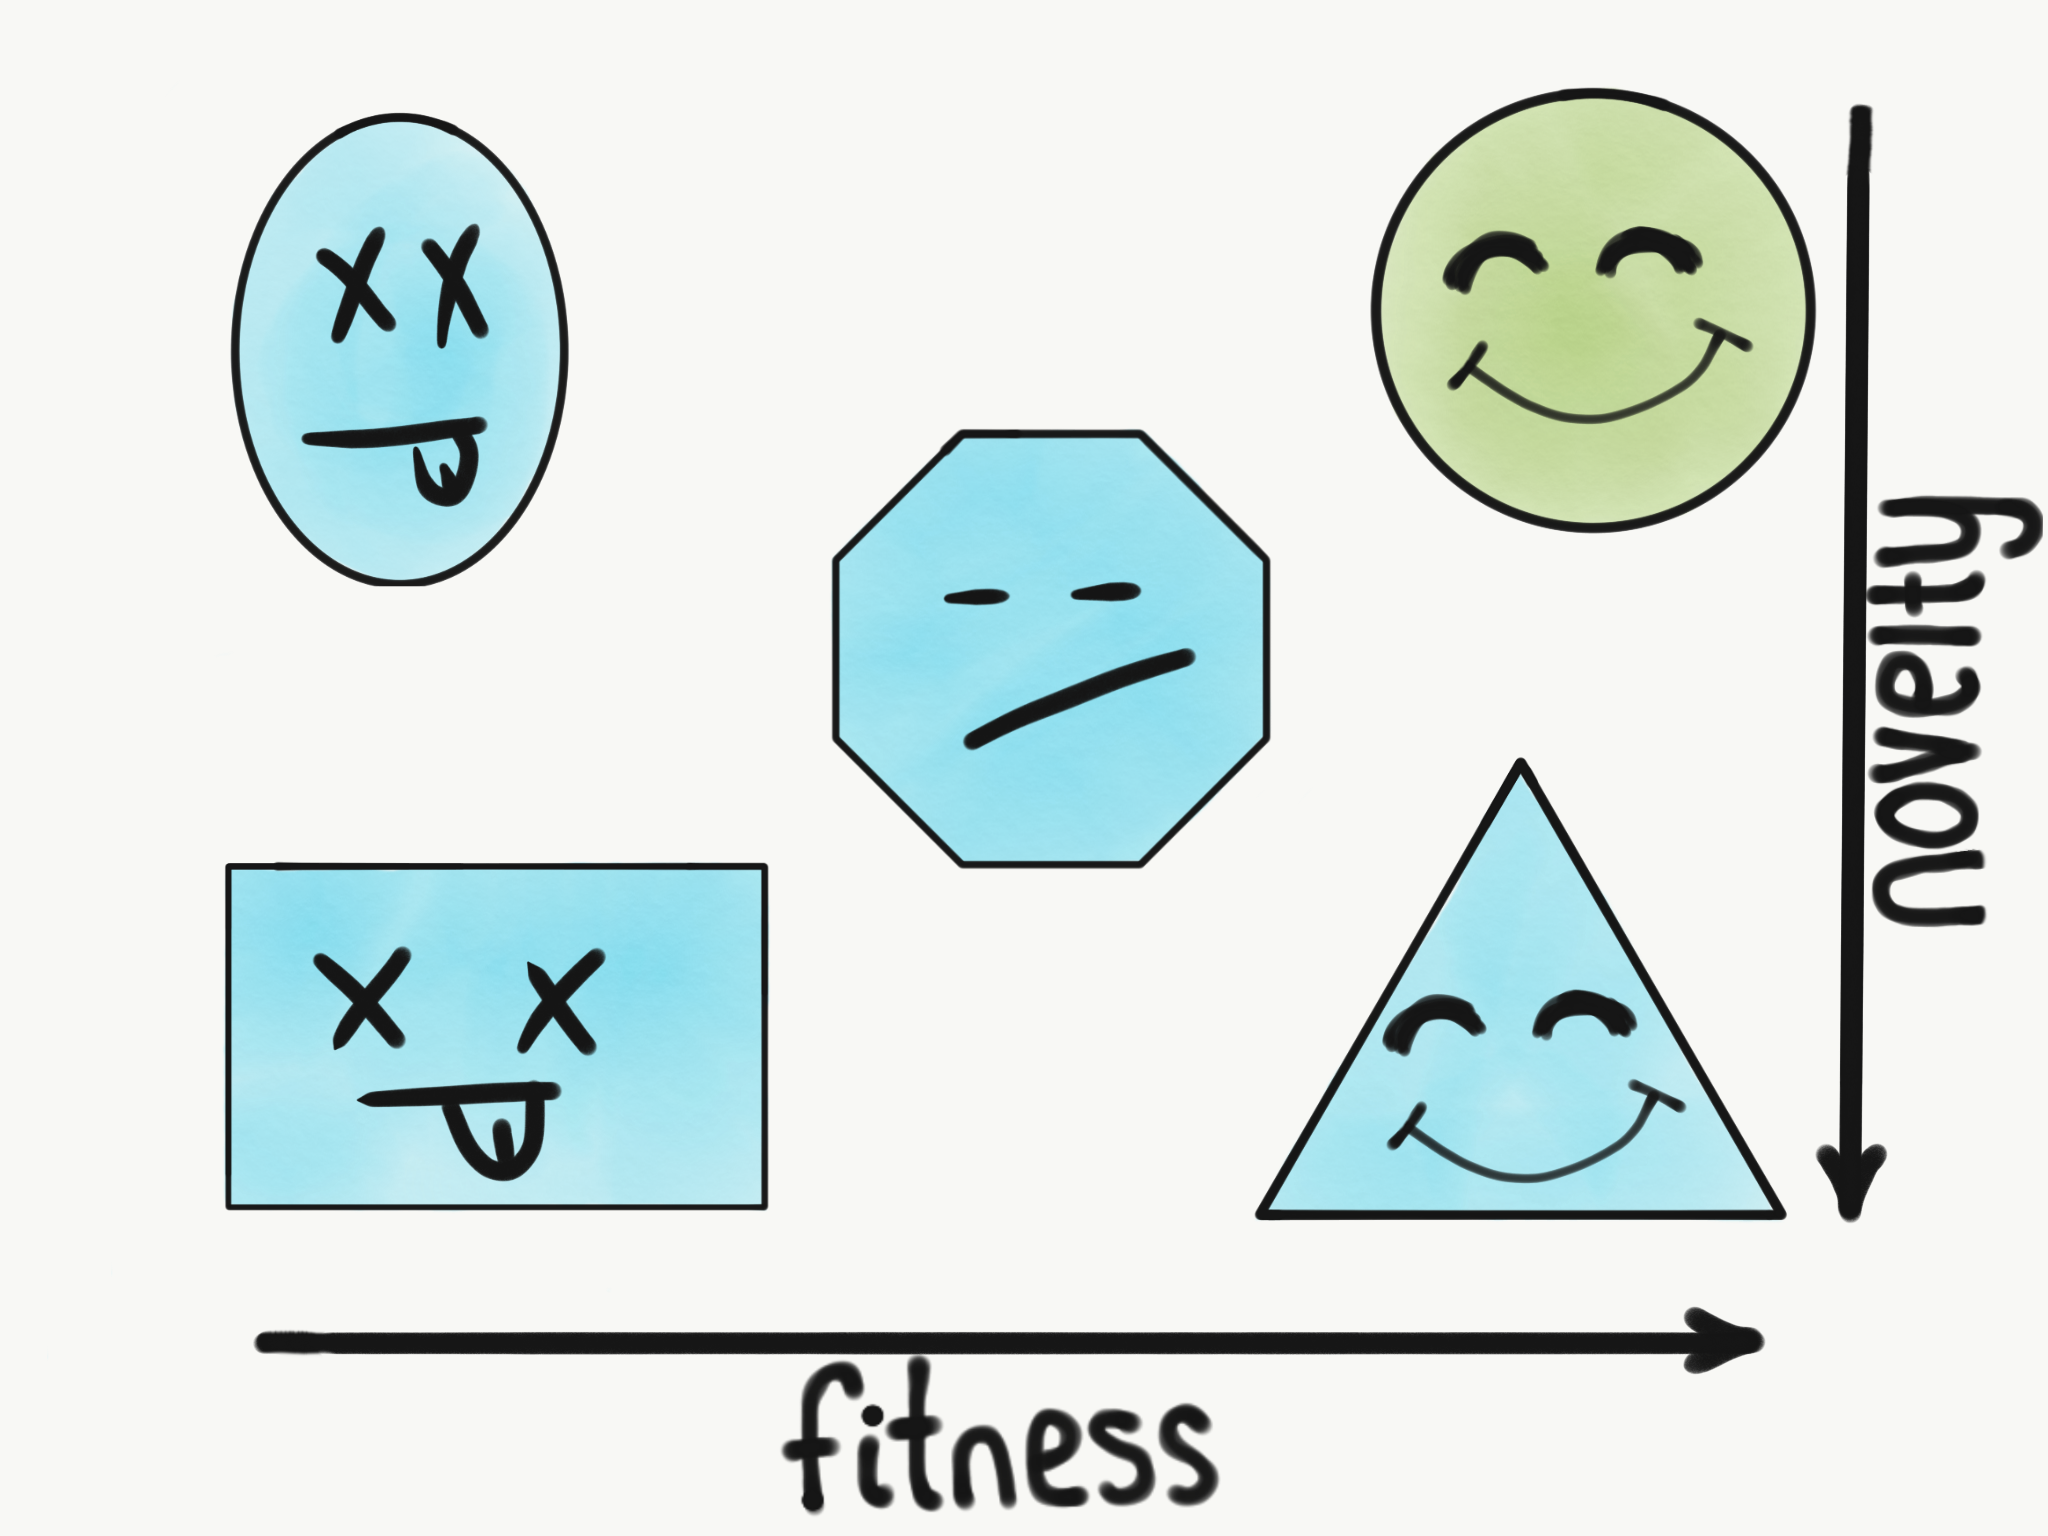
\includegraphics[width=0.8\linewidth]{img/reading_evolvability_signature}
  \caption{
    Cartoon illustration describing the layout of an evolvability signature diagram \cite{tarapore2015evolvability}.
    The parent phenotype is located in the upper right.
    Novelty increases top to bottom and fitness decreases right to left.
  }\label{fig:reading_evolvability_signature}
\end{figure}

